\documentclass[a4paper, 10pt, openany]{book}%标注了文档类型和字号大小
\usepackage{geometry}

\geometry{left=3cm,right=3cm,top=3cm,bottom=3cm}

\usepackage{titlesec}
\usepackage{hyperref}
\usepackage{url} % 用于更好地格式化URL

\titleformat{\section}[block]{\normalfont}{\thesection}{1em}{}
\titleformat{\subsection}[block]{\normalfont}{\thesubsection}{1em}{}
\titleformat{\chapter}[display]
  {\normalfont\huge} % 设置章节标题的字体为正常字体(非加粗)
  {Chapter \thechapter}{1em}{} % 保留 "Chapter" 和 章节编号

\usepackage{xeCJK}
\usepackage{footmisc}
\usepackage[UTF8]{ctex}
\usepackage{amsmath}
\usepackage{subfigure}
\usepackage[graphicx]{realboxes}



\setCJKmainfont{FangSong}%中文设置为仿宋

\setmainfont{Palatino Linotype}%英文设置为palatino linotype

\begin{document}
  \title{ \heiti 分析力学笔记}
  \author{亦可}
  \maketitle
  
 
\tableofcontents


  \newpage

  \chapter{写在前面/Foreword}

%%%%%
嘿嘿,第一章节总是要写的有吸引力些。
\section{写这本笔记的原因}
为什么要写这本笔记?笔者对于这本笔记的全部期望是,它能给第一次接触分
析力学概念的人一个基本的概念。最容易混淆的,笔者并不期望读者通过
这本笔记能够完全掌握分析力学的全部知识(笔者甚至并不期望读者读了这本笔
记就能应付期末考试)。

笔者最初的想法源于,在笔者初入分析力学试图作些预习时,陷入了
找不到合适的参考教材的苦恼(最初,笔者甚至误购了两本偏工科的教材)。国
内的教材中,笔者尝试过刘川老师和梁昆淼老师的《理论力学》
,但是作为初学者,刘川老师的教材过于精炼和抽象,(也许更适合重修理论力
学的同学翻阅。————Friendshao)
这可能是因为刘书本就是从讲义略改而来;梁书则相对中规中矩,也比较全面(
事实上,笔者认为这是中文分析力学教材中比较适合初学者的了)
对于国外教材,读者试图翻开过Landau的《力学》与goldstein的<classical 
mechanics>。Landau力学固然是上品,但是该书的防自学程度相比
刘书过之而无不及(实际上这是合理的,因为学习一门学科的过程中总是
存在一些在作者看来比较幼稚的问题,读者和作者在经验上的巨大差距导致了教
材可读性上的困难)。
笔者认为goldstein的英文原著写的很不错,如果初学者希望挑选一本英文教材的
话,笔者相对更推荐后者。

诸如此类原因吧,笔者试图起到的作用,仅仅是回答一些诸如“分析力学都说了啥”
“这些出现频率很高的方程是咋来的”“这个方程说了啥事”之类的问题。
除此之外,笔者试图在学习的过程中记录自己的一些想法,也许对于初学者来说,
能够有意想不到的效果。
\section{学分析力学的原因}
很经典的问题是,分析力学相较于普物力学有何不同?笔者有理由相信,
大部分物理学的学习者在接触分析力学的概念之前应该已经对普物的力学有了
一定的掌握。既然如此,回答这个问题也就是回答了“为什么我们要学习理论
力学”这个问题。

事实上,在分析“力学”这一领域的问题时,并不存在什么“
只有分析力学才能解决的问题”。如果就到这里,似乎分析力学和力学只是简
单的解题方法上的区别。但是分析力学在物理学中的意义在于,它提供了一个
力学所不具备的,普适性的框架。认真地说, 这种框架并不如普物
力学那样直观,因此对于初学者来说,往往不会从分析力学入门进行物理学习
;但是另一方面,分析力学的优势在于,它的框架对于后续高阶物理课程(eg
.量子、场论、广相etc)有较高的帮助。这就是为什么我们要学习分析力学。
\section{观前提醒}
在撰写本笔记的时候,我们假设你已经掌握了:
\begin{itemize}

\item 数学方面:基本的微积分与线性代数的知识。

\item 物理方面:基本的力学知识,可能会涉及一些电磁学知识。

\end{itemize}
\section{鸣谢与声明}
本笔记基本依附于Friendshao的课程ppt,特此鸣谢。

本笔记完全公开。笔者会持续更新本笔记,如果在阅读中发现可以改进的点,欢迎
与笔者联系!yikezzh@gmail.com

\newpage
\chapter{拉格朗日方程/Lagrange's Equation}
After completing this chapter, you can claim to have studied theoretical mechanics.
\section{广义坐标、约束与自由度}
\subsection{约束}
所谓的约束,就是对你所感兴趣的物理问题所在的空间的描述。所以,约束和约束力的划定不是绝对的,完全取决于你想研究什么问题。

一个经典的例子是固定在三维空间中的弯曲铁丝上紧紧套牢着的光滑圆环。这几乎已
经是一个发生在三维空间的真实的场景(除了“完全固定”“紧紧套牢”和“光滑”),但
是,如果我们只关心圆环在铁丝上的相对位置随时间的变化,那么,这个问题便是一维的。

我们可以将该问题抽象为一个点被固定在一条空间曲线上。曲线方程(2.1)与(2.2)便是描述该空间的约束。\footnote{这里有一个非常关键的点。请注意,约束方程和该方程所代表的“约束作用”不
能同时出现在你的问题中。即,如果你要计算一个与约束A对应的约束力的大小,那么该约
束A就不应当成为你对于问题空间的描述(约束是你对于空间结构的描述,在约束方程已经存
在的情况下讨论约束力,就像是讨论是什么作用使得我们被限制在三维世界)。}
\begin{align}
  f(x,y,z)=0 \\
  g(x,y,z)=0
\end{align}



约束方程为什么会存在?原因是,我们写下的东西太多,而实际上真正的独立的东西太少(
当然,无论是我们自然写下的还是实际上最简洁的,它们都应当保证能够唯一地确定系统的位
形)。想象一个生活在这个曲线上的一维生物,对它们来说,我们写下的约束方程既不能被理解,也没有
产生的必要。可是对我们,更高贵的三维生物,我们显然也可以一眼看出这个问题中只存在一个独
立变量,但是我们有时仍然希望采用三维坐标系来研究,为什么?因为有时候,为了表述问题
中剩余的需要研究的相互作用,多加一些坐标会使得对这些相互作用的研究变得简单(例如本
题中的重力,我们会希望加入竖直方向的坐标以表示之)

不管怎么说,在这种情况下,写下来的变量变多了,为了保证我们研究的问题还是原来的问题,
即空间的维度保持不变,约束方程出现了。



第二,对于更复杂的问题,我们的自以为是也许会稍有变化,例如图[2.1]这个同样经典的例子:
\begin{figure}[ht]
  \centering 
  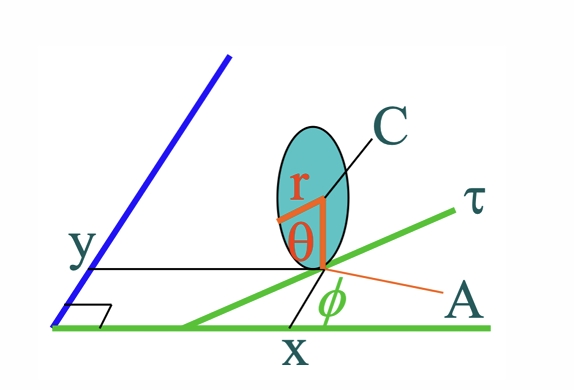
\includegraphics[width=10.5cm]{2.png}
  \caption{}
  \end{figure}

在这个例子中,也许你仍旧随手就写下了四个变量$x, y, \theta, \phi$。但是你也许会不确定,似乎,纯滚条件(2.3)(2.4)也
应当考虑,但是,我们又好像没办法把纯滚条件化作单纯的坐标之间的关系(坐标的时间微分似乎是消不掉的)
由于上述的原因,暂时先写一组并不独立的变量和一些约束方程似乎是合理的。
\begin{align}
  \dot{x}=r\dot{\theta}cos\phi \\
  \dot{y}=r\dot{\theta}sin\phi
\end{align}

约束是可以含时的。在第一个例子中,我们让曲线随时间变化(当然质点仍然固定在曲线上),此时约束就是含时的。
约束是可以含速度的,在第二个例子中,纯滚条件就是含速度的约束。

因此,一个一般的约束可以写为:\footnote{很抱歉,笔者的水平暂时还不能回答,为什么约束方程只到一阶坐标微分这个问题。但是,你可能会发现,一个约束方程对时间求导,会得到一个新的阶数不同的约束(例如x+y=0求导得到x和y方向速度的约束)。一般来说,我们所指称的约束都是尽可能低阶的,因为很显然,低阶的约束包含更强的条件。}
\begin{equation}
  f(\textbf{r}_i,\dot{\textbf{r}}_i,t)=0
\end{equation}

在这里,我们用下标$i$表示第i个质点。
%%%%%

  
  \subsection{约束的分类}
  我们规定,在普适的约束方程(2.5)的基础上,如果约束方程不显含速度,即形如(2.6),或者可以被积分成形如(2.6)的约束被称为完整约束,否则称为非完整约束。
  
  \begin{equation}
    f(\textbf{r}_i,t)=0
  \end{equation}

  定义这个有什么用吗?很有用的。因为直觉上,(至少笔者认为)完整约束是我们更喜欢面对的约束。非完整约束处理起来似乎会麻烦一些(至少,很显然地存在一个问题:我们还没有完全解释清非完整约束对于变量独立性的影响)

  实际上,完整约束减少了独立变量的个数(非常好理解),非完整约束减少了独立坐标微分的个数(不妨随便写下一个非完整约束$v_x+ax+by=0$,整体乘以$\mathrm{d}t$得到$\mathrm{d}x+ax\mathrm{d}t+by\mathrm{d}t=0$,该约束方程表示,在$(x,y)$处,$\mathrm{d}x$和$\mathrm{d}t$之间存在约束关系,因此减少了独立坐标微分的个数)
  
  在(2.5)式的基础上,不含时间的约束,如(2.7)称为稳定约束,否则称为非稳定约束。(“稳定”在这里实际上表现了约束的某种时间特征,例如一个移动的面约束和一个固定的面约束,其区别就在约束的含时上)
  \begin{equation}
    f(\textbf{r}_i,\textbf{v}_i)=0
  \end{equation}
  \subsection{广义坐标与自由度}
  \begin{itemize}
  \item 若一个系统可以用m个独立坐标来唯一确定系统位形,则这组坐标称为一组广义坐标。

  \item 一个系统独立坐标微分的数目是自由度s。
  \end{itemize}
   
   仅有完整约束的时候,广义坐标的数量即为自由度。当一个系统中存在h个非完整约束时,系统的自由度要小于广义坐标的数目,存在关系(2.8)
   \begin{equation}
    h=m-s
   \end{equation}
   

   \subsection{变换方程}

   假设我们已经得到了一组独立坐标,那么,为了将这组坐标与原本我们采用的坐标相联系,我们需要写出它们之间的变换方程。一般的变换方程形如(2.9)所示。
   \begin{equation}
    \textbf{r}_i=\textbf{r}_i(q_j,t)
   \end{equation}

   以及它的微分形式:\footnote{我知道Einstein求和约定很酷,但我们全笔记拒绝使用Einstein求和约定。}

   \begin{equation}
    \mathrm{d}\textbf{r}_i=\frac{\partial \textbf{r}_i}{\partial t}\mathrm{d}t+\sum_{j=1}^s \frac{\partial \textbf{r}_i}{\partial q_j}\mathrm{d}q_j
   \end{equation}
   \section{达朗贝尔原理}
   \label{2.2}
  在讨论这一小节之前,希望你已经看过了关于变分原理的附录\ref{appendix A}。
   \subsection{虚功原理}
   
   等时变分原理,有
   \begin{equation}
    \delta t=0
   \end{equation}
   
   联系上前面微分形式的变换方程(2.10),我们可以得到虚位移的微分(注意,我们用$m$表示广义坐标的个数):
   \begin{equation}
    \delta \textbf{r}_i=\sum_{j=1}^m \frac{\partial \textbf{r}_i}{\partial q_j}\delta q_j
   \end{equation}

   处于平衡状态时,对一个系统有:
   \begin{equation}
   \textbf{F}_i=0
   \end{equation}

   这个方程说明,对于体系中的任意一个质点,其受到的合力都是零。我们把力做一个区分,分为主动力和约束力(请注意,这里的划分并不是唯一的,具体要看你研究的问题而定,一般来说,只要你写出了约束方程,那么就总要存在作用使得质点被束缚,这个作用就是约束方程对应的约束力,我们用$\textbf{F}^D$表示约束力,$\textbf{F}^A$表示主动力),即有:
  
   \begin{equation}
     \textbf{F}^A_i+\textbf{F}^D_i=0
    \end{equation}

   理想约束的定义:
   \begin{equation}
    \sum_{i=1}^n \textbf{F}^D_i\cdot\delta \textbf{r}_i=0
   \end{equation}

请注意,我们在这里第一次将虚位移的概念应用于表达中,所以你应该时刻记得,虚位移不是唯一的,那么理想约束的表达式(2.15)应该对所有可能的虚位移均成立。例如,考虑一个将质点束缚在光滑平面的约束。对于这个约束,显然其约束力是沿着平面法向的,而所有可能的虚位移都平行于平面(请注意,考察虚位移的概念,无论平面处在任何运动中,结果都是相同的),因此显然满足式(2.15),是理想约束。

当然,不只有点乘为零这一种“理想”的方式,也不只有光滑平面这一种理想约束。




   总之,在理想约束下,一个处在平衡状态的系统必然满足:
   \begin{equation}
    \sum_{i=1}^n \textbf{F}^A_i\cdot\delta \textbf{r}_i=0
   \end{equation}
   
   请注意,这里我们已经写出了虚功的表达式(也就是力与任意一个虚位移的点乘),因此这个式子也被称为判定系统平衡的虚功原理。现在我们已经证明,理想约束下(请注意,当我们在讨论一个系统的时候,我们指称“理想约束下”,或是“完整约束下”,我们实际上指的是,这个系统中所有的约束都是理想约束或完整约束),系统平衡能够推出(2.16)式。接下来我们做进一步的推广。


   由(2.12)式,有
   \begin{equation}
    \sum_{i=1}^n(\textbf{F}^A_i \cdot \sum_{j=1}^m \frac{\partial \textbf{r}_i}{\partial q_j}\delta q_j)=0
   \end{equation}
  
   如果我们定义:
   \begin{equation}
   Q_j=\sum_{i=1}^n \textbf{F}_i \cdot \frac{\partial \textbf{r}_i}{\partial q_j}
   \end{equation}

   那么我们就可以得到:
   \begin{equation}
    \sum_{j=1}^m Q_j \delta q_j=0
   \end{equation}
   
   $Q_j$称为广义力。\footnote{请注意,广义力是力和坐标的偏导点乘的结果,因此它不一定仍然具有力的量纲,但有一点肯定的是,广义力与对应坐标维度上虚位移的乘积一定具有能量的量纲。}(2.19)是广义力形式下的虚功原理。完整约束下,$\delta q_j $相互独立,因此为了使(2.19)式成立,应有:
   \begin{equation}
     Q_j=0,j=1,\dots,m
   \end{equation}

   我们现在已经证明,在理想、完整约束下,系统平衡能够推得式(2.20)。

   另一方面,理想约束与稳定约束下,如果有(2.16)式成立,则必然有式(2.21)成立。这是因为,稳定约束下实位移一定属于虚位移。
   \begin{equation}
  \sum_{i=1}^n \textbf{F}_i \cdot\mathrm{d} \textbf{r}_i=0
  \end{equation}
   
   主动力不做功,因此必定保持平衡状态。因此虚功原理的内容:
   一个理想,完整,稳定的系统保持平衡状态,等价于:
   \begin{equation}
    Q_j=0,j=1,\dots,m
   \end{equation}

   这就是虚功原理的广义力形式的表达。
   
   \subsection{达朗贝尔原理}
   系统处于非平衡状态时,由牛顿第二定律有:
   \begin{equation}
   \textbf{F}_i-m\textbf{a}_i=0
   \end{equation}

   上面的式子对体系中每个质点都成立。因此,类似于虚功原理,我们可以构建达朗贝尔原理(注意这个式子不需要任何约束类别限制,是动力学普遍方程):
    
    \begin{equation}
    \sum_{i=1}^n (\textbf{F}_i-m\textbf{a}_i)\cdot \delta \textbf{r}_i=0
    \end{equation}
    
实际上,达朗贝尔原理并没有那么实用。笔者认为,它更像是为了推导拉格朗日方程而做的铺垫准备,因此这里并不花篇幅去介绍达朗贝尔原理。


    \section{拉格朗日方程}
    \subsection{拉格朗日关系}
    拉格朗日关系是为了推导拉格朗日方程做的数学准备。(2.25)和(2.26)分别为第一和第二拉格朗日关系。
    \begin{equation}
        \frac{\partial \textbf{r}_i}{\partial q_j}=\frac{\partial \dot{\textbf{r}}_i}{\partial \dot{q}_j}
    \end{equation}
    
    \begin{equation}
        \frac{\partial \dot{\textbf{r}}_i}{\partial q_j}=\frac{\mathrm{d}}{\mathrm{d}t}\frac{\partial \textbf{r}_i}{\partial q_j}
    \end{equation}

第一拉格朗日关系的推导:
\begin{equation}
\frac{\partial \dot{\textbf{r}}_i}{\partial \dot{q}_j}=\frac{\partial}{\partial \dot{q}_j}\left(\frac{\partial {\textbf{r}}_i}{\partial t}+\sum_{k=1}^m\frac{\partial \textbf{r}_i}{\partial q_k}\dot{q}_k\right)=\frac{\partial \textbf{r}_i}{\partial q_j}
\end{equation}

第二拉格朗日关系的推导:
\begin{equation}
\frac{\partial \dot{\textbf{r}}_i}{\partial {q}_j}=\frac{\partial}{\partial q_j}\left(\frac{\partial {\textbf{r}}_i}{\partial t}+\sum_{k=1}^m\frac{\partial \textbf{r}_i}{\partial q_k}\dot{q}_k\right)=\frac{\partial}{\partial t}\frac{\partial \textbf{r}_i}{\partial q_j}+\sum_{k=1}^m\frac{\partial}{\partial q_k}\left(\frac{\partial \textbf{r}_i}{\partial q_k}\right)\dot{q_k}=\frac{\mathrm{d}}{\mathrm{d}t}\frac{\partial \textbf{r}_i}{\partial q_j}
\end{equation}
    \subsection{牛顿第二定律导出拉氏方程}
    从式(2.24)出发,我们可以进行如下的推导:

    \begin{equation}
    \textbf{func}=\sum_{i=1}^n(\textbf{F}_i-m\ddot{\textbf{r}}_i)\cdot\delta\textbf{r}_i=\sum_{j=1}^mQ_j\delta q_j-\sum_{i=1}^n m_i (\frac{\mathrm{d}}{\mathrm{d}t}(\dot{\textbf{r}}_i\cdot \delta \textbf{r}_i)-\dot{\textbf{r}}_i\cdot \frac{\mathrm{d}}{\mathrm{d}t} \delta \textbf{r}_i)=0
    \end{equation}
    
    将虚位移的表达式代入,我们就可以得到:
    \begin{equation}
    \textbf{func}=\sum_{j=1}^{m}Q_j\delta_j-\sum_{i=1}^n m_i (\frac{\mathrm{d}}{\mathrm{d}t}(\dot{\textbf{r}}_i\cdot (\sum_{j=1}^m \frac{\partial \textbf{r}_i}{\partial q_j}\delta q_j))-\dot{\textbf{r}}_i\cdot \frac{\mathrm{d}}{\mathrm{d}t} (\sum_{j=1}^m \frac{\partial \textbf{r}_i}{\partial q_j}\delta q_j))=0
    \end{equation}
    
    使用两类拉格朗日关系,我们就可以得到:
    \begin{equation}
      \textbf{func}=\sum_{j=1}^{m}Q_j\delta_j-\sum_{i=1}^n m_i (\frac{\mathrm{d}}{\mathrm{d}t}(\dot{\textbf{r}}_i\cdot (\sum_{j=1}^m \frac{\partial \dot{\textbf{r}}_i}{\partial \dot{q}_j}\delta q_j))-\dot{\textbf{r}}_i\cdot (\sum_{j=1}^m \frac{\partial \dot{\textbf{r}}_i}{\partial q_j}\delta q_j))=0
    \end{equation}

    将r点乘放进去,我们就可以得到:
    \begin{equation}
      \textbf{func}=\sum_{j=1}^{m}Q_j\delta_j-\frac{1}{2}\sum_{i=1}^n m_i (\frac{\mathrm{d}}{\mathrm{d}t} (\sum_{j=1}^m \frac{\partial (\dot{\textbf{r}}_i\cdot\dot{\textbf{r}}_i)}{\partial \dot{q}_j}\delta q_j)- (\sum_{j=1}^m \frac{\partial (\dot{\textbf{r}}_i\cdot\dot{\textbf{r}}_i)}{\partial q_j}\delta q_j))=0
    \end{equation}
    
    我们定义动能的表达式(实际上这和普物中的动能是相同的):
    \begin{equation}
        T=\sum_{i=1}^n \frac{1}{2}m_i\sum_{j=1}^m \dot{\textbf{r}}^2_i
    \end{equation}

    于是我们就得到:
    \begin{equation}
        \textbf{func}=\sum_{j=1}^m \left(Q_j-\frac{\mathrm{d}}{\mathrm{d}t}\frac{\partial T}{\partial \dot{q}_j}+\frac{\partial T}{\partial q_j}\right)\delta q_j=0   
          \end{equation}
    
          请注意,直到这里,我们还没有对约束提出要求,因此,直到上面这个方程,都是普适的方程。
    
          当体系中所有的约束都是理想约束时,上式中的$Q_j$可以简化为$Q_j^A$;当体系中所有约束均为完整约束时,我们就得到:

    \begin{equation}
        \frac{\mathrm{d}}{\mathrm{d}t}\frac{\partial T}{\partial \dot{q}_j}-\frac{\partial T}{\partial q_j}=Q_j,j=1,\dots,m
    \end{equation}

    这就是完整约束形式下的拉格朗日方程(组!)。
    
    \subsection{普通有势体系下的拉氏方程}

    很多时候,力的表达式满足某些特征,其中最重要的特征就是力只与位置矢量相关。这种情况下,我们就可以定义势能。(例如重力势能,引力势能等等)普通有势体系中,势能造成的力形如:

    \begin{equation}\textbf{F}=\textbf{F}(\textbf{r},t)\end{equation}
    
    此时可以存在势能函数满足:
    \begin{equation}\textbf{F}=-\nabla V(\textbf{r},t)\end{equation}
    
    请注意,势能函数是可以含时的。这是因为坐标的变换方程可能含时。当你从一组坐标变换到另一组坐标时,可能就会使得势能函数中出现时间项。但是,在广义力的维度下,我们总是可以得到:
    \begin{equation}Q_j=-\frac{\partial V}{\partial q_j}\end{equation}
    
    定义拉格朗日量:
    $$L=T-V$$
    
    我们得到完整约束,有势体系下的拉氏方程:
    \begin{equation}
      \frac{\mathrm{d}}{\mathrm{d}t}\frac{\partial L}{\partial \dot{q}_j}-\frac{\partial L}{\partial q_j}=0
    \end{equation}

    其中$L=L(q_j,\dot{q}_j,t)$。
    注意:得到这个方程的起点是惯性系,因此该拉氏方程需要在惯性系写出。相比于(2.35)式,(2.39)彻底脱离了力的概念,完全用能量来描述方程,因此具有更广泛的推广性。
    \section{拉格朗日量的性质}
    i)描述同一个运动的拉格朗日量可以相差一个常微分,即:
    \begin{equation}
      L^{\prime}=L+\frac{\mathrm{d}}{\mathrm{d}t}u(q_j,t)
    \end{equation}

    这个性质很好被证明,只要把$L^\prime$代入拉格朗日方程你就会明白这个性质的道理。由这个性质
    可知,常数项,仅与时间有关的项等等都不影响运动的形式。实际操作中如何使用这个性质呢?一般来说,只要一个式子能够对$\mathrm{d}t$积分成$u(q_j,t)$的形式,那我们就可以将它添加到拉氏量中(或从拉氏量中删掉它)而不用担心这是否会导致新的拉氏量与之前的拉氏量描述的体系是否存在区别。

    ii)描述同一个运动的拉氏量可以相差一个因子。可以推导出,如果势能项是$\textbf{r}$的$k$阶齐次函数,作变换$t^\prime=\alpha t, \textbf{r}^\prime=\beta\textbf{r}$,则有
    $$L^\prime=(\frac{\beta}{\alpha})^2T-\beta^kV$$
    
    若要求二者描述的是同一运动形式,应有:
    $$\alpha=\beta^{1-\frac{k}{2}}$$
    
    一般来说,$k$是已知的,由力的形式给出,我们可以根据$k$的值来确定系统的力学相似性。
    
    
    \section{广义有势体系}

    从前面的内容可以看出,一般来说,势能只能够写成位移$\textbf{r}$和时间$t$的函数。但是,如果拉格朗日方程(2.35)中的广义力满足:
    
    \begin{equation}Q_j=-\frac{\partial U}{\partial q_j}+\frac{\mathrm{d}}{\mathrm{d}t}\frac{\partial U}{\partial \dot{q}_j}
    \end{equation}

    请注意比对这个方程与(2.38)之间的相似之处。(2.38)式实际上属于上式的一个特例。很显然,既然上式中我们引入了$U$对$\dot{q}_j$的偏导,那么这里的$U$一定也是$\dot{q}_j$的函数。我要表达的是,如果能找到一个$U$,使得$m$个维度上的广义力满足(2.41)式,那么这个$U$也可以类似势能$V$放入拉格朗日方程中,此时$U$被称为广义势能。


    总之大致意思就是,我们放宽了对“可以用一个能够融进拉格朗日方程的势能函数来表示的力”的要求,现在,我们可以把一些原本不能写成势能的力改写成势能并融进拉格朗日方程中。
    
    事实上,整个这套广义势,主要是为了描述电磁力,也就是洛伦兹力。
    \begin{equation}
    \textbf{F}=e\textbf{E}+e\textbf{v}\times\textbf{B}
    \end{equation}

    我们来证明此时存在一个广义势可以满足上述性质,定义$\phi,\textbf{A}${实际上这就是电势和磁矢势}使得
    \begin{equation}\textbf{E}=-\nabla\phi-\frac{\partial \textbf{A}}{\partial t}\end{equation}
    \begin{equation}\textbf{B}=\nabla\times\textbf{A}\end{equation}
    
    此时,洛伦兹力就可以被表示为:
    \begin{equation}\textbf{F}=(-e\nabla\phi-e\frac{\partial \textbf{A}}{\partial t})+e\textbf{v}\times(\nabla\times\textbf{A})\end{equation}
    
    其中有:
  \begin{equation}(\textbf{v}\times(\nabla\times\textbf{A}))_x=v_y(\frac{\partial A_y}{\partial x}-\frac{\partial A_x}{\partial y})-v_z(\frac{\partial A_x}{\partial z}-\frac{\partial A_z}{\partial x})=\frac{\partial}{\partial x}(\textbf{v}\cdot\textbf{A})-(\textbf{v}\cdot\nabla)A_x\end{equation}
    
  经过上式我们完成了一个矢量分析的简单推导,得到了下面这个式子:

    \begin{equation}\textbf{v}\times(\nabla\times\textbf{A})=\nabla(\textbf{v}\cdot\textbf{A})-(\textbf{v}\cdot\nabla)\textbf{A}\end{equation}
    
    带回洛伦兹力的表达式,我们就得到:
    \begin{equation}\textbf{F}=(-e\nabla\phi-e\frac{\partial \textbf{A}}{\partial t})+e(\nabla(\textbf{v}\cdot\textbf{A})-(\textbf{v}\cdot\nabla)\textbf{A})
    \end{equation}

    \begin{equation}\textbf{F}=(-e\nabla(\phi-\textbf{v}\cdot\textbf{A})-e\frac{\partial \textbf{A}}{\partial t})-e(\textbf{v}\cdot\nabla)\textbf{A}
    \end{equation}
    
  
    \begin{equation}\textbf{F}=-e\nabla(\phi-\textbf{v}\cdot\textbf{A})-e\frac{\mathrm{d} \textbf{A}}{\mathrm{d} t}=-e\nabla(\phi-\textbf{v}\cdot\textbf{A})+e\frac{\mathrm{d}}{\mathrm{d} t}\frac{\partial (\phi-\textbf{v}\cdot\textbf{A})}{\partial \textbf{v}}
    \end{equation}

    此时有广义势:
    \begin{equation}U=e(\phi-\textbf{v}\cdot\textbf{A})\end{equation}
    \section{守恒量}

    \subsection{动能函数}
    我们都知道,在力学中,动能被定义为:
    \begin{equation}T=\frac{1}{2}m\sum_{i=1}^n\dot{\textbf{r}}_i^2\end{equation}

    当我们使用广义坐标来表示动能的时候,它就长成了下面这个复杂的样子:
\begin{equation}
T=\frac{1}{2}m\sum_{i=1}^n(\frac{\partial {\textbf{r}}_i}{\partial t}+\sum_{j=1}^m\frac{\partial {\textbf{r}}_i}{\partial q_j}\dot{q}_j)^2
\end{equation}

很显然,我们可以按照广义速度的零、一、二次项对动能函数进行划分,分为$T=T_0+T_1+T_2$。并且,很重要地,零次项和一次项的出现,全都是因为在变换方程组中存在含时的变换方程。但是!需要注意的是,变换方程显含时间,动能函数不一定显含时间。

如果变换方程组不显含时间,我们就可以用矩阵的形式来表述动能,即:
\begin{align}
\dot{\textbf{q}}=(\dot{q}_1,\dots,\dot{q}_m)^T\\
\kappa_{\alpha\beta}=\sum_{i=1}^nm_i\frac{\partial\dot{\textbf{r}}_i}{\partial q_\alpha}\cdot\frac{\partial\dot{\textbf{r}}_i}{\partial q_\beta}\\
\textbf{m}=\begin{pmatrix} \kappa_{11}, \dots, \kappa_{1m}\\
  \dots\\
  \kappa_{m1}, \dots, \kappa_{mm}\end{pmatrix}
\end{align}

此时,动能就可以被表示为:
\begin{equation}
T=\frac{1}{2}\dot{\textbf{q}}^T\textbf{m}\dot{\textbf{q}}
\end{equation}

动能的这种表示方法会在后续章节有比较大的用处,在这里做提及。
\subsection{守恒}

一般来说,如果描述体系运动的某个函数在时间维度上是常量,我们就把这个函数称为运动积分。

如果你把$q_1,\dots,q_m,t$看作$m+1$个维度,那么很有趣的是,对于这$m+1$个坐标,$L$不显含哪一个,就在对应的维度上存在一个运动积分。

   如果$L$不显含某个广义坐标$q_\gamma$,在该方向动量守恒即:
    \begin{equation} p_\gamma=\frac{\partial L}{\partial \dot{q}_j}=C\end{equation}
    
    如果$L$不显含$t$(注意此时势能和动能都不能显含$t$)则有广义能量守恒:
    \begin{equation}T_2-T_0+V=E\end{equation}
    
    这是因为,对任意$q_\gamma$,都有:
    \begin{align}
    \dot{q}_\gamma(\frac{\mathrm{d}}{\mathrm{d}t}\frac{\partial L}{\partial \dot{q}_\gamma}-\frac{\partial L}{\partial q_\gamma})=0\\
    \frac{\mathrm{d}}{\mathrm{d}t}\left(\frac{\partial L}{\partial \dot{q}_\gamma}\dot{q}_\gamma\right)-\frac{\partial L}{\partial \dot{q}_\gamma}\ddot{q}_\gamma-\frac{\partial L}{\partial q_\gamma}\dot{q}_\gamma=0
    \end{align}
    
    与此同时又有:
    \begin{equation}
    \frac{\mathrm{d}L}{\mathrm{d}t}=\sum_{j=1}^m\left(\frac{\partial L}{\partial q_j}\dot{q}_j+\frac{\partial L}{\partial \dot{q}_j}\ddot{q}_j\right)+\frac{\partial L}{\partial t}
    \end{equation}

    $m$个(2.61)方程的和减去(2.62)式,得到:
    \begin{equation}
    \frac{\mathrm{d}}{\mathrm{d}t}\sum_{j=1}^m\left(\frac{\partial L}{\partial \dot{q}_j}\dot{q}_j\right)-\frac{\mathrm{d}L}{\mathrm{d}t}+\frac{\partial L}{\partial t}=0
    \end{equation}

请注意,势能函数中一定不含$\dot{q}$,因此我们得到:
\begin{equation}
\sum_{j=1}^m\frac{\partial L}{\partial \dot{q}_j}\dot{q}_j=(2T_2+T_1)
\end{equation}

因此就有:
\begin{equation}
\frac{\mathrm{d}}{\mathrm{d}t}\left(T_2-T_0+V\right)=0
\end{equation}

得到运动积分。若在此基础上,变换方程与时间有关,则有:
    \begin{equation}T+V=C\end{equation}

    于是我们就讨论了最简单的运动积分。当然,如果运动满足一些其他的形式,可能还会有新的运动积分。运动积分可以代替某些方程来辅助运动的求解,一般来说,作为积分,运动积分是一阶微分方程,相比拉格朗日方程作为二阶微分方程而言更容易求解。
   
 \section{非完整约束下的拉氏方程}
    $$f_k=A_{kj}\dot{q}_j+B_k=0,B=B(q_j,t)$$
    被称为线性非完整约束,遇到线性非完整约束时我们可以使用拉格朗日乘子法进行求解。先由线性非完整约束得到:
    $$\sum_{j=1}^s A_{kj}\delta q_j=0,k=1,\dots,t$$
    $t$个线性非完整约束可以组成一张矩阵$\textbf{A}_{t\times s}$,我们有:
    $$\textbf{A}_{t\times s}(\delta\textbf{ q})=\textbf{0}$$
    拉格朗日乘子法:
    $$\frac{d}{dt}\frac{\partial T}{\partial \dot{q}_j}-\frac{\partial T}{\partial q^j}-Q_j-\sum_{k=1}^t(\lambda_kA_{kj})=0$$
    总是可以选择合适的一组$\lambda_k$使得$k$个自由度上的拉氏方程等于0,于是还剩$s-k$个自由度上的拉氏方程,这些$\delta q_j$都相互独立,因此可以得到$s-k$个拉氏方程,需要注意的是,此时$\lambda_kA_{kj}$为第$k$个约束方程指代的约束力在$q_j$方向的分量。同时,当我们要求完整约束下的某个约束力的时候,也可以采用上述的逻辑,先把完整约束写成线性非完整约束的形式,然后通过拉格朗日乘子法求得之。
     \subsection{耗散}
    $$\textbf{F}=-k\textbf{v}$$
    考虑上述形式的力,要将该耗散力写成主动力的形式,有:
     $$Q_j=\textbf{F}\cdot\frac{\partial \textbf{r}}{\partial q_j}=\textbf{F}\cdot\frac{\partial \dot{\textbf{r}}}{\partial \dot{q}_j}=-k\frac{\partial \dot{\textbf{r}}^2}{\partial \dot{q}_j}$$
    定义耗散函数$\mathcal{F}=\frac{1}{2}k\dot{\textbf{r}}^2$  可以得到:
    $$\frac{d}{dt}\frac{\partial T}{\partial \dot{q}_j}-\frac{\partial T}{\partial q_j}=-\frac{\partial V}{\partial \dot{q}_j}-\frac{\partial \mathcal{F}}{\partial \dot{q}_j}$$
    可以推出:
    $$\frac{d}{dt}(T+V)=-k\textbf{v}^2$$
    \subsection{拉格朗日方程推导牛顿运动定律}
    $$L=L(\textbf{r},\dot{\textbf{r}},t)$$
    考虑自由质点的拉氏量,它应该具有时间对称性,空间对称性和各向同性,故应有:
    $$L=L(\dot{\textbf{r}}^2)$$
    代入拉氏方程有:
    $$\frac{d}{dt}(2\dot{\textbf{r}}\frac{\partial L}{\partial \dot{\textbf{r}}^2})=0$$
    因此自由质点作匀速直线运动,这就是惯性定律。然后我们写出换系之后的拉氏量:
    $$L^\prime=L(\textbf{v}^2)+\frac{\partial L}{\partial \textbf{v}^2}(2\textbf{V}\cdot\textbf{v}+\textbf{V}^2)$$
    已知拉氏量之间只能相差:
    $$\frac{du}{dt}=\frac{\partial u}{\partial t}+\frac{\partial u}{\partial \textbf{r}}\cdot\textbf{v}$$
    因此$L=\alpha\textbf{v}^2$,在经典力学下,通过实验得到的能量值可以得到$L=\frac{1}{2}m\textbf{v}^2$;相对论情形下,有:
    $$S=\int Ldt$$
    为了保证不同参考系的一致性,应有
    $$S=\beta\int ds=\alpha\int c(\sqrt{1-\beta^2})dt$$
    故有:
    $$L=\alpha c \sqrt{1-\beta^2}$$
    动量的推导值$\frac{\partial L}{\partial \textbf{v}}=-\alpha \textbf{v}\gamma/c$,测量值为$\gamma m \textbf{v}$,故相对论下拉氏量为:
    $$L=L=-m c^2 \sqrt{1-\beta^2}$$
    \chapter{有心运动}
    \section{两体问题}
    $$\textbf{r}_c,\textbf{r}_{12}$$
    可以用来表述两体问题中的六个自由度。此时动能有:
    $$T=\frac{1}{2}(m_1+m_2)\dot{\textbf{r}}^2_c+\frac{1}{2}\mu \dot{\textbf{r}}^2_{12}$$
    两体运动中,我们假定:
    $$U=U(t,\textbf{r}_{12},\dot{\textbf{r}}_{12})$$
    故有拉氏量$L=T-U$,可以将这个拉氏量拆成仅与质心相关和仅与相对位置相关的两个新的拉氏量 $L^\prime$和$L^{\prime\prime}$,有:
    $$L^\prime=\frac{1}{2}(m_1+m_2)\dot{\textbf{r}}^2_c,L^{\prime\prime}=\frac{1}{2}\mu \dot{\textbf{r}}^2_{12}-U(t,\textbf{r}_{12},\dot{\textbf{r}}_{12})$$
    后续我们关于$L^{\prime\prime}$进行讨论。事实上,我们可以把该拉氏量看成一个新的粒子的运动,若要求解原运动,我们只需先求解新运动,再利用位移的变换公式就可以推回原运动。大多数情况下,两体运动中有:
    $$U=U(r)$$
    这样的势能和这样的势能对应的力被称为有心势和有心力。若选用球坐标,则可推得:
    $$P_\phi=C,T+U=E,P_\theta=\mu {r}^2\dot{\theta},\frac{dP_\theta}{dt}=\frac{\partial L}{\partial {\theta}}=\mu {r}^2\dot{\phi}sin\theta cos\theta$$
    若我们选择合适的坐标轴,使得初始时$\theta=\pi/2$且$\dot{\theta}=0$,则有$\theta=\pi/2$恒成立。此时广义坐标的数目减为2。
    $$\mu\ddot{r}=\mu r\dot{\phi}^2-\frac{\partial U}{\partial r}$$
    $$\frac{d}{dt}(\mu r^2\dot{\phi})=0$$
    此即我们得到的两个二阶微分方程,或者使用初积分我们可以得到两个一阶微分方程:
    $$\mu r^2\dot{\phi}=J$$
    $$\frac{1}{2}\mu (\dot{r}^2+r^2\dot{\phi}^2)+U=E$$
    引入有效势能:
    $$E_{eff}=U+\frac{J}{2\mu r^2}$$
    即有:
    $$E=\frac{1}{2}\mu \dot{r}^2+E_{eff}$$
    即可解出$r=r(t)$
    \subsection{比奈公式}
    为了求轨道方程$r=r(\phi)$,我们令$C=r^2\dot{\phi},u=1/r$,则有:
    $$\frac{d}{dt}=\dot{\phi}\frac{d}{d\phi}=Cu^2\frac{d}{d\phi}$$
    $$\dot{r}=\frac{dr}{du}\frac{du}{dt}=-\frac{1}{u^2}Cu^2\frac{du}{d\phi}=-C\frac{du}{d\phi}$$
    即能量比奈公式:
    $$\frac{1}{2}\mu C^2((\frac{du}{d\phi})^2+u^2)+U(1/u)=E$$
    不加推导地给出力的比奈公式:
    $$-\mu C^2u^2(\frac{d^2u}{d\phi^2}+u)\textbf{e}_r=\textbf{F}(1/u)$$
    由比奈公式可以得到
    $$\Delta \phi=\int_{u_{min}}^{u_{max}}\frac{du}{\sqrt{(E-U)\frac{2}{\mu C^2}-u^2}}$$
    如果刚好有$2\Delta \phi=2\pi$,则说明轨道闭合,这时候的势能显然拥有更好的对称性。
    \subsection{伯特兰定理}
     $$\Delta \phi=\int_{u_{min}}^{u_{max}}\frac{du}{\sqrt{(E-U)\frac{2}{\mu C^2}-u^2}}$$
    何时轨道闭合且稳定?稳定指径向的微小扰动永远只是径向的微小扰动,不会导致径向运动大的变化(简而言之即径向的微小扰动会产生径向的振动模)考虑函数:
    $$\mathcal{J}=-\frac{\mu}{J^2u^2}F(\frac{1}{u})$$
    考虑相对于圆轨道的微小偏离,即$u=u_0+\delta$,此时$\mathcal{J}=\mathcal{J}_0+\frac{\partial \mathcal{J}}{\partial u}\delta$,由比奈公式有:
    $$\frac{d^2\delta}{d\phi^2}+(1-\frac{\partial \mathcal{J}}{\partial u}_{u=u_0})\delta=0$$
    轨道闭合稳定,这要求$\beta^2=1-\frac{\partial \mathcal{J}}{\partial u}$其中$\beta$应为有理数,则:
    $$\beta^2=1-(\frac{2\mu}{J^2u^3}F(\frac{1}{u})-\frac{\mu}{J^2u^2}\frac{d}{du}(F(\frac{1}{u})))_{u=u_0}$$
    圆轨道时有:
    $$u_0=-\frac{\mu F(\frac{1}{u})}{J^2u^2_0}$$
    即:
    $$\beta^2=3-\frac{u_0}{F(\frac{1}{u_0})}\frac{d}{du}F(\frac{1}{u})$$
    显然$\beta$随$u$连续变化,又有$\beta$为有理数,故有$\beta$为常量,即:
    $$\frac{dF(r)}{dr}=(3-\beta^2)\frac{F(r)}{r}$$
    解得:
    $$F=\alpha r^{3-\beta^2}$$
    此时,稳定等价于:
    $$\beta^2>0$$
    若考虑$\mathcal{J}$的高阶展开,最终可以得到稳定条件:
    $$\beta^2=1,\beta^2=4$$
    分别对应万有引力和谐振子力。
    \subsection{天体运动}
    $$\phi=\int_{u_0}^{u}\frac{du}{\sqrt{(E-U)\frac{2}{\mu C^2}-u^2}}$$
    这里我们考虑万有引力,也就是势能的表达式确定了,并且我们这里考虑中心天体质量足够大的情况,令中心天体的质量为$M_s$定义,当我们需要严格解的时候,只需要记住下述推导中的$m=\mu,M_s=M+m$:
    $$C=r^2\dot{\phi}$$
    $$B=\frac{GM_s}{C^2}$$
    $$A=\sqrt{B^2+\frac{2E}{mC^2}}$$
    $$\phi_0=arcsin(\frac{1-B}{AR})$$
    $B$和$A$的量纲是$1/R$,可以得到天体运动的轨道:
    $$r=\frac{1}{B+Acos(\phi+\phi_0)}$$
    注意:这里$\phi_0$有两个取值(除非$\phi_0=\pm\pi/2$),需要根据发射角来验证。同时,二次曲线的普遍形式$r=\frac{p}{1+ecos({\phi+\phi_0-\frac{\pi}{2}})}$天体运动时有$e=A/B$,$e>1,0<e<1,e=0$分别对应双曲线,椭圆和抛物线。[角动量不变时,圆轨道的能量最小;能量不变时,圆轨道的角动量最大(移动$E_{eff}$的曲线可以得出结论)]
    \subsection{第一、二、三宇宙速度}
    $$v_1=\sqrt{\frac{GM_s}{R}}$$
    $$v_2=\sqrt{2}v_1$$
    $$v_3=\sqrt{(3-2\sqrt{2})\frac{GM_{sun}}{R_{ES}}+\frac{2GM_s}{R}}$$
    \subsection{限制型三体运动}
    $$L=\frac{1}{2}m\dot{\textbf{r}}^2+m\dot{\textbf{r}}\cdot(\Omega \times{\textbf{r}})-V_{eff}$$
    采用转动参考系可以写出如上的拉氏量,其中:
    $$V_{eff}=V_s(\textbf{r}_{sm})+V_e(\textbf{r}_{em})-\frac{1}{2}m\omega^2\textbf{r}_{cm}^2$$
    其中有:
    $$r_{sm}=\sqrt{r^2_{se}+r^2_{em}+2r_{se}r_{em}cos\theta},r_{cm}=\sqrt{r^2_{ce}+r^2_{em}+2r_{ce}r_{em}cos\theta}$$
    注意,离心势能在两种模型下的不同:有心力模型中离心势能为$\frac{1}{2}m\omega^2r^2$但此时$\omega$和$r$并不独立;固定转速情况下的离心势能:$-\frac{1}{2}m\omega^2r^2$。上述有心势能其实是两个自由度,我们不妨认定这两个广义坐标分别为$r_{em}$和$\theta$。则有:
    $$\frac{\partial V_{eff}}{\partial r}=\frac{\partial V_s}{\partial r_{sm}}\frac{r_{em}+r_{se}cos\theta}{r_{sm}}+\frac{\partial V_e}{\partial r_{em}}-m\omega^2(r_{em}+r_{ce}cos\theta)$$
    $$\frac{\partial V_{eff}}{\partial \theta}=-\frac{\partial V_s}{\partial r_{sm}}\frac{r_{se}r_{em}sin\theta}{r_{sm}}+m\omega^2r_{em}r_{ce}sin\theta$$
    关于拉格朗日点和潮汐的问题可以由上两个方程给出
    \subsection{散射}
    $$\textbf{F}=\frac{k}{r^2}\textbf{e}_r,k=\frac{q_1q_2}{4\pi\epsilon_0}$$
    将引力问题中所有的$GM_s$换成$-\frac{k}{\mu}$即可。改变参考系,我们得到瞄准距,会存在近心点和渐近线。实验时我们能看到入射方向与偏转角$\theta$(入射方向与出射方向之间的夹角),有:
    $$\theta=\pi-2arccos\frac{1}{e},cot\frac{\theta}{2}=\sqrt{e^2-1}$$
    直觉:入射速度非常大时偏转角应该非常小(来不及相互作用),带电电荷越大则偏转角越大(同理)。实际操作中,入射速度即能量是可以控制的,真正难以控制的是角动量。故有实际操作中的一一对应关系:
    $$\theta<->e<->b$$
    通过上述关系我们可以探测粒子之间相互作用的形式(卢瑟福$\alpha$粒子—金箔散射实验),显然,由双曲线的知识可知,近心点距离渐近线距离为$b$,又有$a=q_1q_2/8\pi\epsilon_0E$,故存在关系:
    $$b=acot\frac{\theta}{2}$$
    在距离为$b$的窄环金箔面(厚度$l$)上打中的粒子占总粒子比例:$dp=Aln_g\frac{2\pi bdb}{A}$,散射立体角有:$d\Omega=2\pi sin\theta d\theta$,联立有:
    $$p=Aln_g\frac{1}{2A}a^2cot\frac{\theta}{2}\frac{1}{sin^2\frac{\theta}{2}}\frac{d\Omega}{ sin\theta}=ln_g\frac{1}{4}a^2\frac{1}{sin^4\frac{\theta}{2}}{d\Omega}$$
    这里我们忽略了求导时出现的负号,因为我们要的是绝对值。最终,应该有,若有N个粒子入射,则$d\Omega$中的粒子应该有$dN=Ndp(\theta)$,有环形面积$d\sigma=2\pi bdb$,定义微分散射截面:
    $$\sigma_c=\frac{d\sigma}{d\Omega}=\frac{1}{4}a^2\frac{1}{sin^4\frac{\theta}{2}}$$
    这时候微分散射截面的积分:
    $$S=\int_0^\pi\sigma_cd\Omega$$
    发散,这是因为库仑力是长程力。当积分收敛时,可以想象该时的力是一个短程力。此时可以有表征概率的量$\sigma_c/\sigma_T$;另外,靶粒子不固定时,需要考虑实验系和质心系的角度变换关系(此时前推所有都是质心系下的结论)这时有:$tan\theta=\frac{sin\theta^\prime}{cos\theta^\prime+m_1/m_2}$。其中撇系是质心系,$m_1$为撞击粒子的质量,$m_2$为靶粒子的质量。这个结论可以通过经典体系下的能动量关系得出。

\section{小振动}




\newpage

\appendix
\chapter{变分原理/Variational Principle}

\label{appendix A}
考虑函数$f_1(t)$,我们已经了解了它的微分的概念,如(A.1)所示。
\begin{equation}
  df_1=f_1(t+dt)-f_1(t)
\end{equation}

考虑一个新的函数$f_2$,在某一点上,我们可以定义变分如(A.2)所示。\footnote{之所以这里表示为$\delta f_1$而不是$\delta f_2$,是因为我们这里假定$f_2$是由$f_1$变化得到。}

\begin{equation}
  \delta f_1=f_2(t)-f_1(t)
\end{equation}



现在,我们用$y$代替上面的$f_1$,并考虑一个$y$,$y^\prime$和$x$的函数$f=f(y,y^\prime,t)$,现在,我们试图考虑,由于函数$y(t)$变化导致的$f$的变化(因此,这里似乎应该写为$\delta f$而非$df$)。

不过,$f$的表达式并没有改变,从结果上来看,似乎这里与微分的概念很相似:你可以直接把它看成是$t,y,y^\prime$的值发生改变导致$f$的值改变,因此我们得到一个与全微分很像的表达式(A.3)。

\begin{equation}
  \delta f=\frac{\partial f}{\partial y}\delta y+\frac{\partial f}{\partial y^\prime}\delta y^\prime+\frac{\partial f}{\partial t}\delta t
\end{equation}

请注意,这里有一个略微难以理解的点。我没有把握把它讲的很明白。我会先告诉你,在等时变分中,我们规定这里的$\delta t=0$(如果我们用$t$来表示时间)。这是因为,我们研究的是$y(t)$变化的影响,$\delta t$的提法本身就是奇怪的(你会发现我们并没有给出$\delta t$的定义,因为与微分不同,此时$y$的变化并不来自于$t$的变化)。

我来举一个比较直观的例子:想象一个质点被约束在一台电梯的地面上(请注意,我们这里只给出了一个约束,因此质点在该平面上任意的位移都是可能的),电梯正在上升(不妨我们把上升的方向作为$z$轴的正方向)。很显然,经过时间$dt$,质点的任何运动$dx,dy,dz$均有$dz>0$。这就是对于该质点的真实位移的描述。我们把它叫做实位移。显然,实际发生的位移只有一个,所以实位移是唯一的。

现在,让我们从另一个角度来考虑这个运动。随着电梯上升,质点的轨迹会画出一条空间曲线。根据质点相对平面运动形式的不同,它可以画出不同的空间曲线。(请注意联系理解不同空间曲线和不同函数曲线之间的关系)现在,我们来问,在某一个$t_0$时刻,质点采用A轨迹和B轨迹之间的差别是什么?我们用虚位移$\delta \textbf{r}=(\delta x,\delta y,0)$表示这种差别。显然,当我们比较“不同运动轨迹给$f$带来的影响”时,我们总是要比较同一时刻上不同轨迹的差距。因此$\delta t=0$是合理的。同时请注意,由于质点在平面上的运动模式不是唯一的,因此质点在空间中可能的运动轨迹也是无穷多的,所以虚位移是不唯一的。

传送回\ref{2.2}

\end{document}